\documentclass[1p]{elsarticle_modified}
%\bibliographystyle{elsarticle-num}

%\usepackage[colorlinks]{hyperref}
%\usepackage{abbrmath_seonhwa} %\Abb, \Ascr, \Acal ,\Abf, \Afrak
\usepackage{amsfonts}
\usepackage{amssymb}
\usepackage{amsmath}
\usepackage{amsthm}
\usepackage{scalefnt}
\usepackage{amsbsy}
\usepackage{kotex}
\usepackage{caption}
\usepackage{subfig}
\usepackage{color}
\usepackage{graphicx}
\usepackage{xcolor} %% white, black, red, green, blue, cyan, magenta, yellow
\usepackage{float}
\usepackage{setspace}
\usepackage{hyperref}

\usepackage{tikz}
\usetikzlibrary{arrows}

\usepackage{multirow}
\usepackage{array} % fixed length table
\usepackage{hhline}

%%%%%%%%%%%%%%%%%%%%%
\makeatletter
\renewcommand*\env@matrix[1][\arraystretch]{%
	\edef\arraystretch{#1}%
	\hskip -\arraycolsep
	\let\@ifnextchar\new@ifnextchar
	\array{*\c@MaxMatrixCols c}}
\makeatother %https://tex.stackexchange.com/questions/14071/how-can-i-increase-the-line-spacing-in-a-matrix
%%%%%%%%%%%%%%%

\usepackage[normalem]{ulem}

\newcommand{\msout}[1]{\ifmmode\text{\sout{\ensuremath{#1}}}\else\sout{#1}\fi}
%SOURCE: \msout is \stkout macro in https://tex.stackexchange.com/questions/20609/strikeout-in-math-mode

\newcommand{\cancel}[1]{
	\ifmmode
	{\color{red}\msout{#1}}
	\else
	{\color{red}\sout{#1}}
	\fi
}

\newcommand{\add}[1]{
	{\color{blue}\uwave{#1}}
}

\newcommand{\replace}[2]{
	\ifmmode
	{\color{red}\msout{#1}}{\color{blue}\uwave{#2}}
	\else
	{\color{red}\sout{#1}}{\color{blue}\uwave{#2}}
	\fi
}

\newcommand{\Sol}{\mathcal{S}} %segment
\newcommand{\D}{D} %diagram
\newcommand{\A}{\mathcal{A}} %arc


%%%%%%%%%%%%%%%%%%%%%%%%%%%%%5 test

\def\sl{\operatorname{\textup{SL}}(2,\Cbb)}
\def\psl{\operatorname{\textup{PSL}}(2,\Cbb)}
\def\quan{\mkern 1mu \triangleright \mkern 1mu}

\theoremstyle{definition}
\newtheorem{thm}{Theorem}[section]
\newtheorem{prop}[thm]{Proposition}
\newtheorem{lem}[thm]{Lemma}
\newtheorem{ques}[thm]{Question}
\newtheorem{cor}[thm]{Corollary}
\newtheorem{defn}[thm]{Definition}
\newtheorem{exam}[thm]{Example}
\newtheorem{rmk}[thm]{Remark}
\newtheorem{alg}[thm]{Algorithm}

\newcommand{\I}{\sqrt{-1}}
\begin{document}

%\begin{frontmatter}
%
%\title{Boundary parabolic representations of knots up to 8 crossings}
%
%%% Group authors per affiliation:
%\author{Yunhi Cho} 
%\address{Department of Mathematics, University of Seoul, Seoul, Korea}
%\ead{yhcho@uos.ac.kr}
%
%
%\author{Seonhwa Kim} %\fnref{s_kim}}
%\address{Center for Geometry and Physics, Institute for Basic Science, Pohang, 37673, Korea}
%\ead{ryeona17@ibs.re.kr}
%
%\author{Hyuk Kim}
%\address{Department of Mathematical Sciences, Seoul National University, Seoul 08826, Korea}
%\ead{hyukkim@snu.ac.kr}
%
%\author{Seokbeom Yoon}
%\address{Department of Mathematical Sciences, Seoul National University, Seoul, 08826,  Korea}
%\ead{sbyoon15@snu.ac.kr}
%
%\begin{abstract}
%We find all boundary parabolic representation of knots up to 8 crossings.
%
%\end{abstract}
%\begin{keyword}
%    \MSC[2010] 57M25 
%\end{keyword}
%
%\end{frontmatter}

%\linenumbers
%\tableofcontents
%
\newcommand\colored[1]{\textcolor{white}{\rule[-0.35ex]{0.8em}{1.4ex}}\kern-0.8em\color{red} #1}%
%\newcommand\colored[1]{\textcolor{white}{ #1}\kern-2.17ex	\textcolor{white}{ #1}\kern-1.81ex	\textcolor{white}{ #1}\kern-2.15ex\color{red}#1	}

{\Large $\underline{12n_{0650}~(K12n_{0650})}$}

\setlength{\tabcolsep}{10pt}
\renewcommand{\arraystretch}{1.6}
\vspace{1cm}\begin{tabular}{m{100pt}>{\centering\arraybackslash}m{274pt}}
\multirow{5}{120pt}{
	\centering
	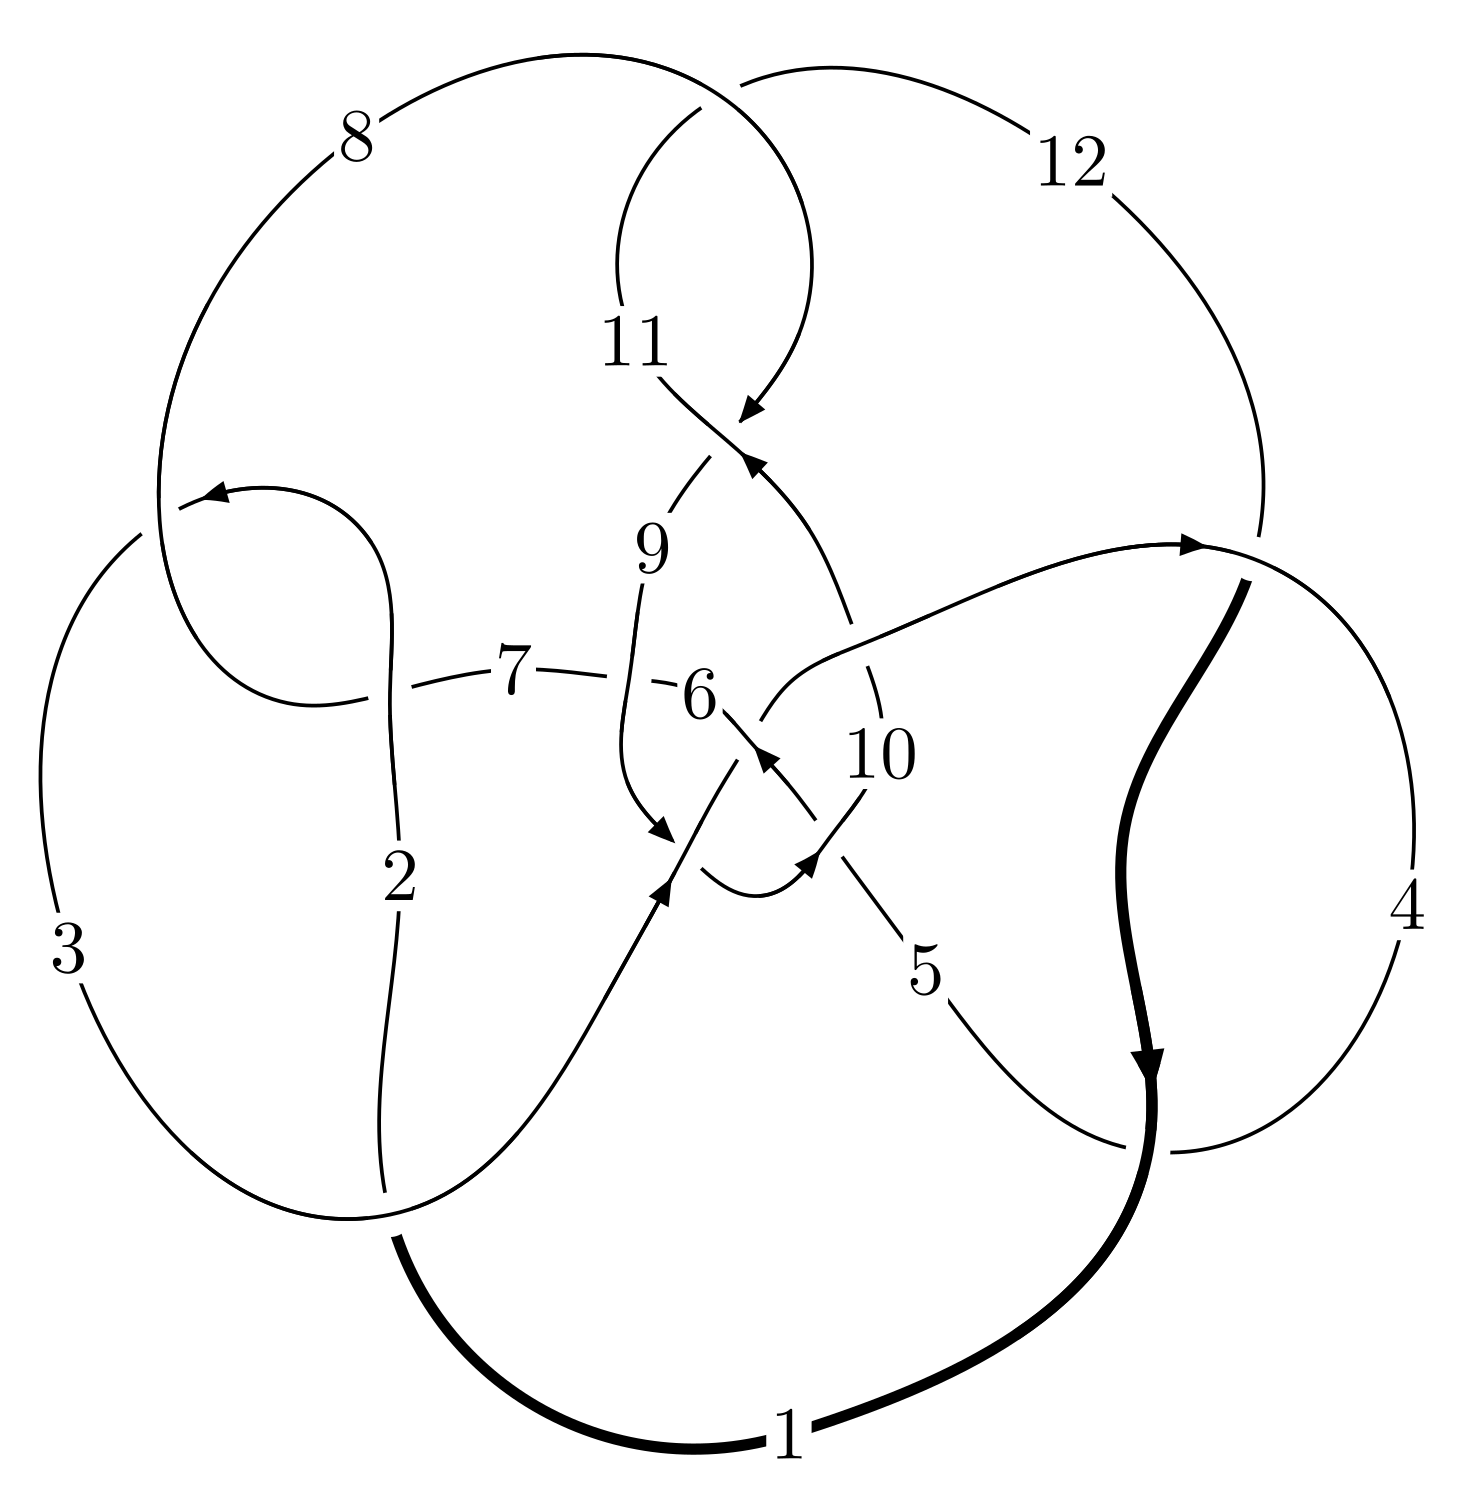
\includegraphics[width=112pt]{../../../GIT/diagram.site/Diagrams/png/2739_12n_0650.png}\\
\ \ \ A knot diagram\footnotemark}&
\allowdisplaybreaks
\textbf{Linearized knot diagam} \\
\cline{2-2}
 &
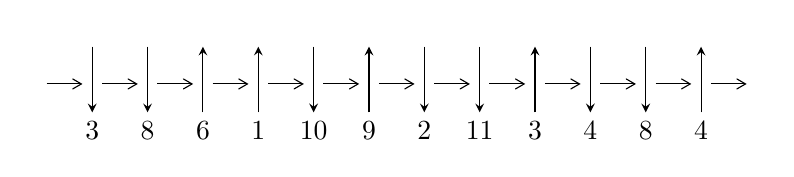
\begin{tikzpicture}[x=20pt, y=17pt]
	% nodes
	\node (C0) at (0, 0) {};
	\node (C1) at (1, 0) {};
	\node (C1U) at (1, +1) {};
	\node (C1D) at (1, -1) {3};

	\node (C2) at (2, 0) {};
	\node (C2U) at (2, +1) {};
	\node (C2D) at (2, -1) {8};

	\node (C3) at (3, 0) {};
	\node (C3U) at (3, +1) {};
	\node (C3D) at (3, -1) {6};

	\node (C4) at (4, 0) {};
	\node (C4U) at (4, +1) {};
	\node (C4D) at (4, -1) {1};

	\node (C5) at (5, 0) {};
	\node (C5U) at (5, +1) {};
	\node (C5D) at (5, -1) {10};

	\node (C6) at (6, 0) {};
	\node (C6U) at (6, +1) {};
	\node (C6D) at (6, -1) {9};

	\node (C7) at (7, 0) {};
	\node (C7U) at (7, +1) {};
	\node (C7D) at (7, -1) {2};

	\node (C8) at (8, 0) {};
	\node (C8U) at (8, +1) {};
	\node (C8D) at (8, -1) {11};

	\node (C9) at (9, 0) {};
	\node (C9U) at (9, +1) {};
	\node (C9D) at (9, -1) {3};

	\node (C10) at (10, 0) {};
	\node (C10U) at (10, +1) {};
	\node (C10D) at (10, -1) {4};

	\node (C11) at (11, 0) {};
	\node (C11U) at (11, +1) {};
	\node (C11D) at (11, -1) {8};

	\node (C12) at (12, 0) {};
	\node (C12U) at (12, +1) {};
	\node (C12D) at (12, -1) {4};
	\node (C13) at (13, 0) {};

	% arrows
	\draw[->,>={angle 60}]
	(C0) edge (C1) (C1) edge (C2) (C2) edge (C3) (C3) edge (C4) (C4) edge (C5) (C5) edge (C6) (C6) edge (C7) (C7) edge (C8) (C8) edge (C9) (C9) edge (C10) (C10) edge (C11) (C11) edge (C12) (C12) edge (C13) ;	\draw[->,>=stealth]
	(C1U) edge (C1D) (C2U) edge (C2D) (C3D) edge (C3U) (C4D) edge (C4U) (C5U) edge (C5D) (C6D) edge (C6U) (C7U) edge (C7D) (C8U) edge (C8D) (C9D) edge (C9U) (C10U) edge (C10D) (C11U) edge (C11D) (C12D) edge (C12U) ;
	\end{tikzpicture} \\
\hhline{~~} \\& 
\textbf{Solving Sequence} \\ \cline{2-2} 
 &
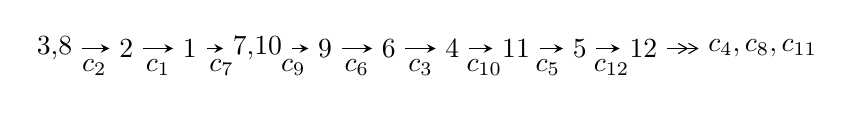
\begin{tikzpicture}[x=23pt, y=7pt]
	% node
	\node (A0) at (-1/8, 0) {3,8};
	\node (A1) at (1, 0) {2};
	\node (A2) at (2, 0) {1};
	\node (A3) at (49/16, 0) {7,10};
	\node (A4) at (33/8, 0) {9};
	\node (A5) at (41/8, 0) {6};
	\node (A6) at (49/8, 0) {4};
	\node (A7) at (57/8, 0) {11};
	\node (A8) at (65/8, 0) {5};
	\node (A9) at (73/8, 0) {12};
	\node (C1) at (1/2, -1) {$c_{2}$};
	\node (C2) at (3/2, -1) {$c_{1}$};
	\node (C3) at (5/2, -1) {$c_{7}$};
	\node (C4) at (29/8, -1) {$c_{9}$};
	\node (C5) at (37/8, -1) {$c_{6}$};
	\node (C6) at (45/8, -1) {$c_{3}$};
	\node (C7) at (53/8, -1) {$c_{10}$};
	\node (C8) at (61/8, -1) {$c_{5}$};
	\node (C9) at (69/8, -1) {$c_{12}$};
	\node (A10) at (11, 0) {$c_{4},c_{8},c_{11}$};

	% edge
	\draw[->,>=stealth]	
	(A0) edge (A1) (A1) edge (A2) (A2) edge (A3) (A3) edge (A4) (A4) edge (A5) (A5) edge (A6) (A6) edge (A7) (A7) edge (A8) (A8) edge (A9) ;
	\draw[->>,>={angle 60}]	
	(A9) edge (A10);
\end{tikzpicture} \\ 

\end{tabular} \\

\footnotetext{
The image of knot diagram is generated by the software ``\textbf{Draw programme}" developed by Andrew Bartholomew(\url{http://www.layer8.co.uk/maths/draw/index.htm\#Running-draw}), where we modified some parts for our purpose(\url{https://github.com/CATsTAILs/LinksPainter}).
}\phantom \\ \newline 
\centering \textbf{Ideals for irreducible components\footnotemark of $X_{\text{par}}$} 
 
\begin{align*}
I^u_{1}&=\langle 
-1989385 u^{25}-36760790 u^{24}+\cdots+9723136 b-272866048,\\
\phantom{I^u_{1}}&\phantom{= \langle  }-3511211 u^{25}-66741367 u^{24}+\cdots+9723136 a-730323648,\;u^{26}+20 u^{25}+\cdots+1536 u+256\rangle \\
I^u_{2}&=\langle 
1174 u^{17}+443 u^{16}+\cdots+2225 b-946,\;13156 u^{17}+10017 u^{16}+\cdots+6675 a-37699,\\
\phantom{I^u_{2}}&\phantom{= \langle  }u^{18}-8 u^{16}+\cdots+5 u+3\rangle \\
\\
\end{align*}
\raggedright * 2 irreducible components of $\dim_{\mathbb{C}}=0$, with total 44 representations.\\
\footnotetext{All coefficients of polynomials are rational numbers. But the coefficients are sometimes approximated in decimal forms when there is not enough margin.}
\newpage
\renewcommand{\arraystretch}{1}
\centering \section*{I. $I^u_{1}= \langle -1.99\times10^{6} u^{25}-3.68\times10^{7} u^{24}+\cdots+9.72\times10^{6} b-2.73\times10^{8},\;-3.51\times10^{6} u^{25}-6.67\times10^{7} u^{24}+\cdots+9.72\times10^{6} a-7.30\times10^{8},\;u^{26}+20 u^{25}+\cdots+1536 u+256 \rangle$}
\flushleft \textbf{(i) Arc colorings}\\
\begin{tabular}{m{7pt} m{180pt} m{7pt} m{180pt} }
\flushright $a_{3}=$&$\begin{pmatrix}1\\0\end{pmatrix}$ \\
\flushright $a_{8}=$&$\begin{pmatrix}0\\u\end{pmatrix}$ \\
\flushright $a_{2}=$&$\begin{pmatrix}1\\- u^2\end{pmatrix}$ \\
\flushright $a_{1}=$&$\begin{pmatrix}- u^2+1\\- u^2\end{pmatrix}$ \\
\flushright $a_{7}=$&$\begin{pmatrix}u\\- u^3+u\end{pmatrix}$ \\
\flushright $a_{10}=$&$\begin{pmatrix}0.361119 u^{25}+6.86418 u^{24}+\cdots+406.596 u+75.1119\\0.204603 u^{25}+3.78075 u^{24}+\cdots+161.401 u+28.0636\end{pmatrix}$ \\
\flushright $a_{9}=$&$\begin{pmatrix}0.156516 u^{25}+3.08343 u^{24}+\cdots+245.195 u+47.0484\\0.204603 u^{25}+3.78075 u^{24}+\cdots+161.401 u+28.0636\end{pmatrix}$ \\
\flushright $a_{6}=$&$\begin{pmatrix}0.110888 u^{25}+2.05128 u^{24}+\cdots+135.662 u+27.3983\\-0.168663 u^{25}-3.00422 u^{24}+\cdots-83.4070 u-14.2327\end{pmatrix}$ \\
\flushright $a_{4}=$&$\begin{pmatrix}0.132026 u^{25}+2.48277 u^{24}+\cdots+132.959 u+25.2820\\0.306676 u^{25}+5.66909 u^{24}+\cdots+248.834 u+44.7104\end{pmatrix}$ \\
\flushright $a_{11}=$&$\begin{pmatrix}-0.0156496 u^{25}-0.512299 u^{24}+\cdots-170.823 u-36.1491\\-0.731644 u^{25}-13.8490 u^{24}+\cdots-665.992 u-115.163\end{pmatrix}$ \\
\flushright $a_{5}=$&$\begin{pmatrix}0.168353 u^{25}+3.05304 u^{24}+\cdots+177.060 u+35.1491\\0.500752 u^{25}+9.22376 u^{24}+\cdots+470.444 u+88.3760\end{pmatrix}$ \\
\flushright $a_{12}=$&$\begin{pmatrix}0.0156496 u^{25}+0.512299 u^{24}+\cdots+170.823 u+36.1491\\0.266199 u^{25}+5.25708 u^{24}+\cdots+355.852 u+64.1406\end{pmatrix}$\\&\end{tabular}
\flushleft \textbf{(ii) Obstruction class $= -1$}\\~\\
\flushleft \textbf{(iii) Cusp Shapes $= -\frac{1519127}{151924} u^{25}-\frac{228486283}{1215392} u^{24}+\cdots-\frac{399437504}{37981} u-\frac{3997508}{1999}$}\\~\\
\newpage\renewcommand{\arraystretch}{1}
\flushleft \textbf{(iv) u-Polynomials at the component}\newline \\
\begin{tabular}{m{50pt}|m{274pt}}
Crossings & \hspace{64pt}u-Polynomials at each crossing \\
\hline $$\begin{aligned}c_{1}\end{aligned}$$&$\begin{aligned}
&u^{26}+16 u^{25}+\cdots+65536 u+65536
\end{aligned}$\\
\hline $$\begin{aligned}c_{2},c_{7}\end{aligned}$$&$\begin{aligned}
&u^{26}-20 u^{25}+\cdots-1536 u+256
\end{aligned}$\\
\hline $$\begin{aligned}c_{3}\end{aligned}$$&$\begin{aligned}
&u^{26}+3 u^{25}+\cdots+5 u+1
\end{aligned}$\\
\hline $$\begin{aligned}c_{4},c_{12}\end{aligned}$$&$\begin{aligned}
&u^{26}+u^{25}+\cdots-2 u+1
\end{aligned}$\\
\hline $$\begin{aligned}c_{5}\end{aligned}$$&$\begin{aligned}
&u^{26}+u^{25}+\cdots+217 u+193
\end{aligned}$\\
\hline $$\begin{aligned}c_{6},c_{9}\end{aligned}$$&$\begin{aligned}
&u^{26}+2 u^{25}+\cdots+2 u+1
\end{aligned}$\\
\hline $$\begin{aligned}c_{8},c_{11}\end{aligned}$$&$\begin{aligned}
&u^{26}-4 u^{25}+\cdots-6 u+1
\end{aligned}$\\
\hline $$\begin{aligned}c_{10}\end{aligned}$$&$\begin{aligned}
&u^{26}+24 u^{24}+\cdots+107 u+43
\end{aligned}$\\
\hline
\end{tabular}\\~\\
\newpage\renewcommand{\arraystretch}{1}
\flushleft \textbf{(v) Riley Polynomials at the component}\newline \\
\begin{tabular}{m{50pt}|m{274pt}}
Crossings & \hspace{64pt}Riley Polynomials at each crossing \\
\hline $$\begin{aligned}c_{1}\end{aligned}$$&$\begin{aligned}
&y^{26}+120 y^{25}+\cdots+122406567936 y+4294967296
\end{aligned}$\\
\hline $$\begin{aligned}c_{2},c_{7}\end{aligned}$$&$\begin{aligned}
&y^{26}-16 y^{25}+\cdots-65536 y+65536
\end{aligned}$\\
\hline $$\begin{aligned}c_{3}\end{aligned}$$&$\begin{aligned}
&y^{26}+3 y^{25}+\cdots+13 y+1
\end{aligned}$\\
\hline $$\begin{aligned}c_{4},c_{12}\end{aligned}$$&$\begin{aligned}
&y^{26}-47 y^{25}+\cdots-2 y+1
\end{aligned}$\\
\hline $$\begin{aligned}c_{5}\end{aligned}$$&$\begin{aligned}
&y^{26}+53 y^{25}+\cdots+99205 y+37249
\end{aligned}$\\
\hline $$\begin{aligned}c_{6},c_{9}\end{aligned}$$&$\begin{aligned}
&y^{26}-54 y^{25}+\cdots-2 y+1
\end{aligned}$\\
\hline $$\begin{aligned}c_{8},c_{11}\end{aligned}$$&$\begin{aligned}
&y^{26}+30 y^{24}+\cdots+2 y+1
\end{aligned}$\\
\hline $$\begin{aligned}c_{10}\end{aligned}$$&$\begin{aligned}
&y^{26}+48 y^{25}+\cdots+3085 y+1849
\end{aligned}$\\
\hline
\end{tabular}\\~\\
\newpage\flushleft \textbf{(vi) Complex Volumes and Cusp Shapes}
$$\begin{array}{c|c|c}  
\text{Solutions to }I^u_{1}& \I (\text{vol} + \sqrt{-1}CS) & \text{Cusp shape}\\
 \hline 
\begin{aligned}
u &= -1.016860 + 0.515617 I \\
a &= -0.547952 - 0.593599 I \\
b &= -0.005131 - 0.349931 I\end{aligned}
 & \phantom{-}1.14259 + 4.55293 I & \phantom{-}0.67584 - 2.96671 I \\ \hline\begin{aligned}
u &= -1.016860 - 0.515617 I \\
a &= -0.547952 + 0.593599 I \\
b &= -0.005131 + 0.349931 I\end{aligned}
 & \phantom{-}1.14259 - 4.55293 I & \phantom{-}0.67584 + 2.96671 I \\ \hline\begin{aligned}
u &= -0.367875 + 0.728872 I \\
a &= -0.726824 + 0.229748 I \\
b &= -0.305544 + 0.145494 I\end{aligned}
 & \phantom{-}1.79332 - 1.76675 I & \phantom{-}0.88475 + 2.70026 I \\ \hline\begin{aligned}
u &= -0.367875 - 0.728872 I \\
a &= -0.726824 - 0.229748 I \\
b &= -0.305544 - 0.145494 I\end{aligned}
 & \phantom{-}1.79332 + 1.76675 I & \phantom{-}0.88475 - 2.70026 I \\ \hline\begin{aligned}
u &= -0.527735 + 0.607198 I \\
a &= -0.345868 - 0.800773 I \\
b &= -0.121889 - 0.310496 I\end{aligned}
 & \phantom{-}2.58885 - 0.08583 I & \phantom{-}6.93906 - 0.29216 I \\ \hline\begin{aligned}
u &= -0.527735 - 0.607198 I \\
a &= -0.345868 + 0.800773 I \\
b &= -0.121889 + 0.310496 I\end{aligned}
 & \phantom{-}2.58885 + 0.08583 I & \phantom{-}6.93906 + 0.29216 I \\ \hline\begin{aligned}
u &= \phantom{-}1.203720 + 0.288453 I \\
a &= \phantom{-}0.465886 + 0.245129 I \\
b &= \phantom{-}0.749365 + 0.223786 I\end{aligned}
 & -2.65605 - 1.02761 I & -3.38805 + 0.66160 I \\ \hline\begin{aligned}
u &= \phantom{-}1.203720 - 0.288453 I \\
a &= \phantom{-}0.465886 - 0.245129 I \\
b &= \phantom{-}0.749365 - 0.223786 I\end{aligned}
 & -2.65605 + 1.02761 I & -3.38805 - 0.66160 I \\ \hline\begin{aligned}
u &= -1.102930 + 0.577266 I \\
a &= \phantom{-}0.450976 - 0.348600 I \\
b &= \phantom{-}0.295113 + 0.026156 I\end{aligned}
 & -0.34242 + 6.74821 I & \phantom{-}1.68908 - 12.55727 I \\ \hline\begin{aligned}
u &= -1.102930 - 0.577266 I \\
a &= \phantom{-}0.450976 + 0.348600 I \\
b &= \phantom{-}0.295113 - 0.026156 I\end{aligned}
 & -0.34242 - 6.74821 I & \phantom{-}1.68908 + 12.55727 I\\
 \hline 
 \end{array}$$\newpage$$\begin{array}{c|c|c}  
\text{Solutions to }I^u_{1}& \I (\text{vol} + \sqrt{-1}CS) & \text{Cusp shape}\\
 \hline 
\begin{aligned}
u &= \phantom{-}0.296079 + 0.669488 I \\
a &= -1.52910 + 0.28993 I \\
b &= -0.675653 + 0.872173 I\end{aligned}
 & -0.13239 - 2.18215 I & -1.31091 + 4.66032 I \\ \hline\begin{aligned}
u &= \phantom{-}0.296079 - 0.669488 I \\
a &= -1.52910 - 0.28993 I \\
b &= -0.675653 - 0.872173 I\end{aligned}
 & -0.13239 + 2.18215 I & -1.31091 - 4.66032 I \\ \hline\begin{aligned}
u &= -1.398550 + 0.175389 I \\
a &= \phantom{-}0.859045 - 0.438947 I \\
b &= \phantom{-}0.029505 + 1.040670 I\end{aligned}
 & -6.70940 + 3.17946 I & -11.81324 + 0. I\phantom{ +0.000000I} \\ \hline\begin{aligned}
u &= -1.398550 - 0.175389 I \\
a &= \phantom{-}0.859045 + 0.438947 I \\
b &= \phantom{-}0.029505 - 1.040670 I\end{aligned}
 & -6.70940 - 3.17946 I & -11.81324 + 0. I\phantom{ +0.000000I} \\ \hline\begin{aligned}
u &= -1.42731 + 0.24870 I \\
a &= \phantom{-}1.005720 - 0.776152 I \\
b &= \phantom{-}0.774240 + 1.177450 I\end{aligned}
 & -5.69335 + 5.51976 I & \phantom{-0.000000 } 0. - 13.25882 I \\ \hline\begin{aligned}
u &= -1.42731 - 0.24870 I \\
a &= \phantom{-}1.005720 + 0.776152 I \\
b &= \phantom{-}0.774240 - 1.177450 I\end{aligned}
 & -5.69335 - 5.51976 I & \phantom{-0.000000 -}0. + 13.25882 I \\ \hline\begin{aligned}
u &= \phantom{-}0.407621 + 0.360624 I \\
a &= -0.738146 + 0.444980 I \\
b &= \phantom{-}0.212985 + 0.764335 I\end{aligned}
 & -1.12681 - 1.09104 I & -5.44567 + 3.98120 I \\ \hline\begin{aligned}
u &= \phantom{-}0.407621 - 0.360624 I \\
a &= -0.738146 - 0.444980 I \\
b &= \phantom{-}0.212985 - 0.764335 I\end{aligned}
 & -1.12681 + 1.09104 I & -5.44567 - 3.98120 I \\ \hline\begin{aligned}
u &= -1.44306 + 1.35548 I \\
a &= \phantom{-}3.43426 - 0.14475 I \\
b &= \phantom{-}2.80277 + 0.65564 I\end{aligned}
 & \phantom{-}14.1380 + 5.5276 I & \phantom{-0.000000 } 0 \\ \hline\begin{aligned}
u &= -1.44306 - 1.35548 I \\
a &= \phantom{-}3.43426 + 0.14475 I \\
b &= \phantom{-}2.80277 - 0.65564 I\end{aligned}
 & \phantom{-}14.1380 - 5.5276 I & \phantom{-0.000000 } 0\\
 \hline 
 \end{array}$$\newpage$$\begin{array}{c|c|c}  
\text{Solutions to }I^u_{1}& \I (\text{vol} + \sqrt{-1}CS) & \text{Cusp shape}\\
 \hline 
\begin{aligned}
u &= -1.56135 + 1.29391 I \\
a &= -3.52741 - 0.39308 I \\
b &= -2.83872 - 1.22660 I\end{aligned}
 & \phantom{-}13.8077 + 5.1544 I & \phantom{-0.000000 } 0 \\ \hline\begin{aligned}
u &= -1.56135 - 1.29391 I \\
a &= -3.52741 + 0.39308 I \\
b &= -2.83872 + 1.22660 I\end{aligned}
 & \phantom{-}13.8077 - 5.1544 I & \phantom{-0.000000 } 0 \\ \hline\begin{aligned}
u &= -1.52058 + 1.37669 I \\
a &= \phantom{-}3.67620 + 0.32681 I \\
b &= \phantom{-}2.97403 + 1.10938 I\end{aligned}
 & \phantom{-}13.8209 + 12.8202 I & \phantom{-0.000000 } 0 \\ \hline\begin{aligned}
u &= -1.52058 - 1.37669 I \\
a &= \phantom{-}3.67620 - 0.32681 I \\
b &= \phantom{-}2.97403 - 1.10938 I\end{aligned}
 & \phantom{-}13.8209 - 12.8202 I & \phantom{-0.000000 } 0 \\ \hline\begin{aligned}
u &= -1.54118 + 1.38126 I \\
a &= -3.47680 - 0.05371 I \\
b &= -2.89107 - 0.84018 I\end{aligned}
 & \phantom{-}13.78230 - 1.84091 I & \phantom{-0.000000 } 0 \\ \hline\begin{aligned}
u &= -1.54118 - 1.38126 I \\
a &= -3.47680 + 0.05371 I \\
b &= -2.89107 + 0.84018 I\end{aligned}
 & \phantom{-}13.78230 + 1.84091 I & \phantom{-0.000000 } 0\\
 \hline 
 \end{array}$$\newpage\newpage\renewcommand{\arraystretch}{1}
\centering \section*{II. $I^u_{2}= \langle 1174 u^{17}+443 u^{16}+\cdots+2225 b-946,\;13156 u^{17}+10017 u^{16}+\cdots+6675 a-37699,\;u^{18}-8 u^{16}+\cdots+5 u+3 \rangle$}
\flushleft \textbf{(i) Arc colorings}\\
\begin{tabular}{m{7pt} m{180pt} m{7pt} m{180pt} }
\flushright $a_{3}=$&$\begin{pmatrix}1\\0\end{pmatrix}$ \\
\flushright $a_{8}=$&$\begin{pmatrix}0\\u\end{pmatrix}$ \\
\flushright $a_{2}=$&$\begin{pmatrix}1\\- u^2\end{pmatrix}$ \\
\flushright $a_{1}=$&$\begin{pmatrix}- u^2+1\\- u^2\end{pmatrix}$ \\
\flushright $a_{7}=$&$\begin{pmatrix}u\\- u^3+u\end{pmatrix}$ \\
\flushright $a_{10}=$&$\begin{pmatrix}-1.97094 u^{17}-1.50067 u^{16}+\cdots+18.7823 u+5.64779\\-0.527640 u^{17}-0.199101 u^{16}+\cdots+1.60135 u+0.425169\end{pmatrix}$ \\
\flushright $a_{9}=$&$\begin{pmatrix}-1.44330 u^{17}-1.30157 u^{16}+\cdots+17.1810 u+5.22262\\-0.527640 u^{17}-0.199101 u^{16}+\cdots+1.60135 u+0.425169\end{pmatrix}$ \\
\flushright $a_{6}=$&$\begin{pmatrix}-0.390712 u^{17}+0.369888 u^{16}+\cdots+2.98816 u+0.0235206\\0.185169 u^{17}-0.0970787 u^{16}+\cdots+3.65438 u+2.28180\end{pmatrix}$ \\
\flushright $a_{4}=$&$\begin{pmatrix}-0.419925 u^{17}+0.996854 u^{16}+\cdots-10.5714 u-4.42142\\1.27910 u^{17}-0.282247 u^{16}+\cdots-1.02337 u+5.09708\end{pmatrix}$ \\
\flushright $a_{11}=$&$\begin{pmatrix}-0.149513 u^{17}-0.960449 u^{16}+\cdots+6.32599 u+5.44075\\-1.02472 u^{17}+0.838202 u^{16}+\cdots-3.24270 u-6.53034\end{pmatrix}$ \\
\flushright $a_{5}=$&$\begin{pmatrix}0.326592 u^{17}+0.683146 u^{16}+\cdots-11.6419 u-4.20524\\1.02876 u^{17}-0.248090 u^{16}+\cdots+0.227865 u+4.05348\end{pmatrix}$ \\
\flushright $a_{12}=$&$\begin{pmatrix}-0.149513 u^{17}-0.960449 u^{16}+\cdots+6.32599 u+5.44075\\-1.36584 u^{17}+0.405393 u^{16}+\cdots+2.00809 u-3.64899\end{pmatrix}$\\&\end{tabular}
\flushleft \textbf{(ii) Obstruction class $= 1$}\\~\\
\flushleft \textbf{(iii) Cusp Shapes $= \frac{8359}{2225} u^{17}+\frac{13288}{2225} u^{16}+\cdots-\frac{127808}{2225} u-\frac{6186}{2225}$}\\~\\
\newpage\renewcommand{\arraystretch}{1}
\flushleft \textbf{(iv) u-Polynomials at the component}\newline \\
\begin{tabular}{m{50pt}|m{274pt}}
Crossings & \hspace{64pt}u-Polynomials at each crossing \\
\hline $$\begin{aligned}c_{1}\end{aligned}$$&$\begin{aligned}
&u^{18}-16 u^{17}+\cdots-109 u+9
\end{aligned}$\\
\hline $$\begin{aligned}c_{2}\end{aligned}$$&$\begin{aligned}
&u^{18}-8 u^{16}+\cdots+5 u+3
\end{aligned}$\\
\hline $$\begin{aligned}c_{3}\end{aligned}$$&$\begin{aligned}
&u^{18}+8 u^{17}+\cdots+5 u+1
\end{aligned}$\\
\hline $$\begin{aligned}c_{4}\end{aligned}$$&$\begin{aligned}
&u^{18}+2 u^{17}+\cdots+2 u+1
\end{aligned}$\\
\hline $$\begin{aligned}c_{5}\end{aligned}$$&$\begin{aligned}
&u^{18}+2 u^{14}+\cdots- u+3
\end{aligned}$\\
\hline $$\begin{aligned}c_{6},c_{9}\end{aligned}$$&$\begin{aligned}
&u^{18}- u^{17}+\cdots+2 u+1
\end{aligned}$\\
\hline $$\begin{aligned}c_{7}\end{aligned}$$&$\begin{aligned}
&u^{18}-8 u^{16}+\cdots-5 u+3
\end{aligned}$\\
\hline $$\begin{aligned}c_{8}\end{aligned}$$&$\begin{aligned}
&u^{18}-9 u^{17}+\cdots-6 u+1
\end{aligned}$\\
\hline $$\begin{aligned}c_{10}\end{aligned}$$&$\begin{aligned}
&u^{18}- u^{17}+\cdots+u+1
\end{aligned}$\\
\hline $$\begin{aligned}c_{11}\end{aligned}$$&$\begin{aligned}
&u^{18}+9 u^{17}+\cdots+6 u+1
\end{aligned}$\\
\hline $$\begin{aligned}c_{12}\end{aligned}$$&$\begin{aligned}
&u^{18}-2 u^{17}+\cdots-2 u+1
\end{aligned}$\\
\hline
\end{tabular}\\~\\
\newpage\renewcommand{\arraystretch}{1}
\flushleft \textbf{(v) Riley Polynomials at the component}\newline \\
\begin{tabular}{m{50pt}|m{274pt}}
Crossings & \hspace{64pt}Riley Polynomials at each crossing \\
\hline $$\begin{aligned}c_{1}\end{aligned}$$&$\begin{aligned}
&y^{18}-16 y^{17}+\cdots- y+81
\end{aligned}$\\
\hline $$\begin{aligned}c_{2},c_{7}\end{aligned}$$&$\begin{aligned}
&y^{18}-16 y^{17}+\cdots-109 y+9
\end{aligned}$\\
\hline $$\begin{aligned}c_{3}\end{aligned}$$&$\begin{aligned}
&y^{18}+2 y^{17}+\cdots+9 y+1
\end{aligned}$\\
\hline $$\begin{aligned}c_{4},c_{12}\end{aligned}$$&$\begin{aligned}
&y^{18}+2 y^{15}+\cdots+2 y+1
\end{aligned}$\\
\hline $$\begin{aligned}c_{5}\end{aligned}$$&$\begin{aligned}
&y^{18}+4 y^{16}+\cdots-7 y+9
\end{aligned}$\\
\hline $$\begin{aligned}c_{6},c_{9}\end{aligned}$$&$\begin{aligned}
&y^{18}+y^{17}+\cdots+2 y+1
\end{aligned}$\\
\hline $$\begin{aligned}c_{8},c_{11}\end{aligned}$$&$\begin{aligned}
&y^{18}- y^{17}+\cdots-2 y+1
\end{aligned}$\\
\hline $$\begin{aligned}c_{10}\end{aligned}$$&$\begin{aligned}
&y^{18}- y^{17}+\cdots+y+1
\end{aligned}$\\
\hline
\end{tabular}\\~\\
\newpage\flushleft \textbf{(vi) Complex Volumes and Cusp Shapes}
$$\begin{array}{c|c|c}  
\text{Solutions to }I^u_{2}& \I (\text{vol} + \sqrt{-1}CS) & \text{Cusp shape}\\
 \hline 
\begin{aligned}
u &= -0.866748 + 0.339139 I \\
a &= \phantom{-}0.585312 - 0.000404 I \\
b &= \phantom{-}0.850307 + 0.487196 I\end{aligned}
 & \phantom{-}1.52696 + 5.64075 I & \phantom{-}5.02271 - 10.09643 I \\ \hline\begin{aligned}
u &= -0.866748 - 0.339139 I \\
a &= \phantom{-}0.585312 + 0.000404 I \\
b &= \phantom{-}0.850307 - 0.487196 I\end{aligned}
 & \phantom{-}1.52696 - 5.64075 I & \phantom{-}5.02271 + 10.09643 I \\ \hline\begin{aligned}
u &= \phantom{-}0.835918 + 0.396708 I \\
a &= \phantom{-}1.08228 + 1.91732 I \\
b &= \phantom{-}0.572770 + 0.331333 I\end{aligned}
 & -3.84181 + 1.43571 I & -2.77803 + 0.44283 I \\ \hline\begin{aligned}
u &= \phantom{-}0.835918 - 0.396708 I \\
a &= \phantom{-}1.08228 - 1.91732 I \\
b &= \phantom{-}0.572770 - 0.331333 I\end{aligned}
 & -3.84181 - 1.43571 I & -2.77803 - 0.44283 I \\ \hline\begin{aligned}
u &= -0.556480 + 0.956948 I \\
a &= \phantom{-}0.659533 + 0.994382 I \\
b &= \phantom{-}0.138758 + 1.050230 I\end{aligned}
 & \phantom{-}1.155690 + 0.058941 I & -0.908103 - 0.566791 I \\ \hline\begin{aligned}
u &= -0.556480 - 0.956948 I \\
a &= \phantom{-}0.659533 - 0.994382 I \\
b &= \phantom{-}0.138758 - 1.050230 I\end{aligned}
 & \phantom{-}1.155690 - 0.058941 I & -0.908103 + 0.566791 I \\ \hline\begin{aligned}
u &= \phantom{-}0.765456 + 0.230677 I \\
a &= -0.44776 - 3.06535 I \\
b &= -0.332709 - 0.567316 I\end{aligned}
 & -2.87507 - 5.25661 I & \phantom{-}0.15175 + 7.52339 I \\ \hline\begin{aligned}
u &= \phantom{-}0.765456 - 0.230677 I \\
a &= -0.44776 + 3.06535 I \\
b &= -0.332709 + 0.567316 I\end{aligned}
 & -2.87507 + 5.25661 I & \phantom{-}0.15175 - 7.52339 I \\ \hline\begin{aligned}
u &= -1.142420 + 0.682096 I \\
a &= -0.060431 + 0.661371 I \\
b &= -0.317939 + 0.747295 I\end{aligned}
 & -0.62367 + 6.19450 I & -4.05821 - 1.05531 I \\ \hline\begin{aligned}
u &= -1.142420 - 0.682096 I \\
a &= -0.060431 - 0.661371 I \\
b &= -0.317939 - 0.747295 I\end{aligned}
 & -0.62367 - 6.19450 I & -4.05821 + 1.05531 I\\
 \hline 
 \end{array}$$\newpage$$\begin{array}{c|c|c}  
\text{Solutions to }I^u_{2}& \I (\text{vol} + \sqrt{-1}CS) & \text{Cusp shape}\\
 \hline 
\begin{aligned}
u &= -1.354680 + 0.072381 I \\
a &= -1.003230 + 0.341552 I \\
b &= -1.47456 + 0.43997 I\end{aligned}
 & -0.97412 - 3.24688 I & -2.87279 + 2.26909 I \\ \hline\begin{aligned}
u &= -1.354680 - 0.072381 I \\
a &= -1.003230 - 0.341552 I \\
b &= -1.47456 - 0.43997 I\end{aligned}
 & -0.97412 + 3.24688 I & -2.87279 - 2.26909 I \\ \hline\begin{aligned}
u &= -0.544801 + 0.244143 I \\
a &= -0.114341 - 0.566988 I \\
b &= \phantom{-}0.906433 - 0.354928 I\end{aligned}
 & \phantom{-}3.11907 - 2.19821 I & \phantom{-}8.90400 + 3.10341 I \\ \hline\begin{aligned}
u &= -0.544801 - 0.244143 I \\
a &= -0.114341 + 0.566988 I \\
b &= \phantom{-}0.906433 + 0.354928 I\end{aligned}
 & \phantom{-}3.11907 + 2.19821 I & \phantom{-}8.90400 - 3.10341 I \\ \hline\begin{aligned}
u &= \phantom{-}1.38521 + 0.32967 I \\
a &= -1.44449 - 0.77157 I \\
b &= -0.87794 + 1.14508 I\end{aligned}
 & -5.93825 - 5.17067 I & -10.95523 - 1.48147 I \\ \hline\begin{aligned}
u &= \phantom{-}1.38521 - 0.32967 I \\
a &= -1.44449 + 0.77157 I \\
b &= -0.87794 - 1.14508 I\end{aligned}
 & -5.93825 + 5.17067 I & -10.95523 + 1.48147 I \\ \hline\begin{aligned}
u &= \phantom{-}1.47855 + 0.08650 I \\
a &= -0.423539 - 0.429164 I \\
b &= \phantom{-}0.034873 + 1.260500 I\end{aligned}
 & -6.35322 - 3.65803 I & -3.50609 + 6.99719 I \\ \hline\begin{aligned}
u &= \phantom{-}1.47855 - 0.08650 I \\
a &= -0.423539 + 0.429164 I \\
b &= \phantom{-}0.034873 - 1.260500 I\end{aligned}
 & -6.35322 + 3.65803 I & -3.50609 - 6.99719 I\\
 \hline 
 \end{array}$$\newpage
\newpage\renewcommand{\arraystretch}{1}
\centering \section*{ III. u-Polynomials}
\begin{tabular}{m{50pt}|m{274pt}}
Crossings & \hspace{64pt}u-Polynomials at each crossing \\
\hline $$\begin{aligned}c_{1}\end{aligned}$$&$\begin{aligned}
&(u^{18}-16 u^{17}+\cdots-109 u+9)(u^{26}+16 u^{25}+\cdots+65536 u+65536)
\end{aligned}$\\
\hline $$\begin{aligned}c_{2}\end{aligned}$$&$\begin{aligned}
&(u^{18}-8 u^{16}+\cdots+5 u+3)(u^{26}-20 u^{25}+\cdots-1536 u+256)
\end{aligned}$\\
\hline $$\begin{aligned}c_{3}\end{aligned}$$&$\begin{aligned}
&(u^{18}+8 u^{17}+\cdots+5 u+1)(u^{26}+3 u^{25}+\cdots+5 u+1)
\end{aligned}$\\
\hline $$\begin{aligned}c_{4}\end{aligned}$$&$\begin{aligned}
&(u^{18}+2 u^{17}+\cdots+2 u+1)(u^{26}+u^{25}+\cdots-2 u+1)
\end{aligned}$\\
\hline $$\begin{aligned}c_{5}\end{aligned}$$&$\begin{aligned}
&(u^{18}+2 u^{14}+\cdots- u+3)(u^{26}+u^{25}+\cdots+217 u+193)
\end{aligned}$\\
\hline $$\begin{aligned}c_{6},c_{9}\end{aligned}$$&$\begin{aligned}
&(u^{18}- u^{17}+\cdots+2 u+1)(u^{26}+2 u^{25}+\cdots+2 u+1)
\end{aligned}$\\
\hline $$\begin{aligned}c_{7}\end{aligned}$$&$\begin{aligned}
&(u^{18}-8 u^{16}+\cdots-5 u+3)(u^{26}-20 u^{25}+\cdots-1536 u+256)
\end{aligned}$\\
\hline $$\begin{aligned}c_{8}\end{aligned}$$&$\begin{aligned}
&(u^{18}-9 u^{17}+\cdots-6 u+1)(u^{26}-4 u^{25}+\cdots-6 u+1)
\end{aligned}$\\
\hline $$\begin{aligned}c_{10}\end{aligned}$$&$\begin{aligned}
&(u^{18}- u^{17}+\cdots+u+1)(u^{26}+24 u^{24}+\cdots+107 u+43)
\end{aligned}$\\
\hline $$\begin{aligned}c_{11}\end{aligned}$$&$\begin{aligned}
&(u^{18}+9 u^{17}+\cdots+6 u+1)(u^{26}-4 u^{25}+\cdots-6 u+1)
\end{aligned}$\\
\hline $$\begin{aligned}c_{12}\end{aligned}$$&$\begin{aligned}
&(u^{18}-2 u^{17}+\cdots-2 u+1)(u^{26}+u^{25}+\cdots-2 u+1)
\end{aligned}$\\
\hline
\end{tabular}\newpage\renewcommand{\arraystretch}{1}
\centering \section*{ IV. Riley Polynomials}
\begin{tabular}{m{50pt}|m{274pt}}
Crossings & \hspace{64pt}Riley Polynomials at each crossing \\
\hline $$\begin{aligned}c_{1}\end{aligned}$$&$\begin{aligned}
&(y^{18}-16 y^{17}+\cdots- y+81)\\
&\cdot(y^{26}+120 y^{25}+\cdots+122406567936 y+4294967296)
\end{aligned}$\\
\hline $$\begin{aligned}c_{2},c_{7}\end{aligned}$$&$\begin{aligned}
&(y^{18}-16 y^{17}+\cdots-109 y+9)(y^{26}-16 y^{25}+\cdots-65536 y+65536)
\end{aligned}$\\
\hline $$\begin{aligned}c_{3}\end{aligned}$$&$\begin{aligned}
&(y^{18}+2 y^{17}+\cdots+9 y+1)(y^{26}+3 y^{25}+\cdots+13 y+1)
\end{aligned}$\\
\hline $$\begin{aligned}c_{4},c_{12}\end{aligned}$$&$\begin{aligned}
&(y^{18}+2 y^{15}+\cdots+2 y+1)(y^{26}-47 y^{25}+\cdots-2 y+1)
\end{aligned}$\\
\hline $$\begin{aligned}c_{5}\end{aligned}$$&$\begin{aligned}
&(y^{18}+4 y^{16}+\cdots-7 y+9)(y^{26}+53 y^{25}+\cdots+99205 y+37249)
\end{aligned}$\\
\hline $$\begin{aligned}c_{6},c_{9}\end{aligned}$$&$\begin{aligned}
&(y^{18}+y^{17}+\cdots+2 y+1)(y^{26}-54 y^{25}+\cdots-2 y+1)
\end{aligned}$\\
\hline $$\begin{aligned}c_{8},c_{11}\end{aligned}$$&$\begin{aligned}
&(y^{18}- y^{17}+\cdots-2 y+1)(y^{26}+30 y^{24}+\cdots+2 y+1)
\end{aligned}$\\
\hline $$\begin{aligned}c_{10}\end{aligned}$$&$\begin{aligned}
&(y^{18}- y^{17}+\cdots+y+1)(y^{26}+48 y^{25}+\cdots+3085 y+1849)
\end{aligned}$\\
\hline
\end{tabular}
\vskip 2pc
\end{document}